\documentclass[9pt]{acm_proc_article-sp}
\usepackage{graphicx}
\usepackage{amsmath}
\usepackage{enumerate}
\usepackage{multirow}
\usepackage{epstopdf}
\usepackage{array}
\usepackage{CJK}
\usepackage{float}
\usepackage{subfigure}
\usepackage{algorithm}
\usepackage{algorithmicx}
\newcommand{\algorithmicbreak}{\textbf{break}}
\newcommand{\BREAK}{\State \algorithmicbreak}
\usepackage{algpseudocode}
\begin{document}

\conferenceinfo{WWW}{'15 Companion, May 18-22, 2015, Florence, Italy}
\title{AVER: Random Walk Based Academic Venue Recommendation}

\numberofauthors{1}
\author{
% 1st. author
\alignauthor
Zhen Chen, Huizhen Jiang, Haifeng Liu, Jun Zhang, Feng Xia\\
       \affaddr{School of Software, Dalian University of Technology, Dalian 116620, China}\\
       \email{f.xia@acm.org}
%% 2nd. author
%\alignauthor
%G.K.M. Tobin\titlenote{The secretary disavows
%any knowledge of this author's actions.}\\
%       \affaddr{Institute for Clarity in Documentation}\\
%       \affaddr{P.O. Box 1212}\\
%       \affaddr{Dublin, Ohio 43017-6221}\\
%       \email{webmaster@marysville-ohio.com}
%% 3rd. author
%\alignauthor Lars Th{\o}rv{\"a}ld\titlenote{This author is the
%one who did all the really hard work.}\\
%       \affaddr{The Th{\o}rv{\"a}ld Group}\\
%       \affaddr{1 Th{\o}rv{\"a}ld Circle}\\
%       \affaddr{Hekla, Iceland}\\
%       \email{larst@affiliation.org}
%\and  % use '\and' if you need 'another row' of author names
%% 4th. author
%\alignauthor Lawrence P. Leipuner\\
%       \affaddr{Brookhaven Laboratories}\\
%       \affaddr{Brookhaven National Lab}\\
%       \affaddr{P.O. Box 5000}\\
%       \email{lleipuner@researchlabs.org}
%% 5th. author
%\alignauthor Sean Fogarty\\
%       \affaddr{NASA Ames Research Center}\\
%       \affaddr{Moffett Field}\\
%       \affaddr{California 94035}\\
%       \email{fogartys@amesres.org}
%% 6th. author
%\alignauthor Charles Palmer\\
%       \affaddr{Palmer Research Laboratories}\\
%       \affaddr{8600 Datapoint Drive}\\
%       \affaddr{San Antonio, Texas 78229}\\
%       \email{cpalmer@prl.com}
}
% There's nothing stopping you putting the seventh, eighth, etc.
% author on the opening page (as the 'third row') but we ask,
% for aesthetic reasons that you place these 'additional authors'
% in the \additional authors block, viz.
%\additionalauthors{Additional authors: John Smith (The Th{\o}rv{\"a}ld Group,
%email: {\texttt{jsmith@affiliation.org}}) and Julius P.~Kumquat
%(The Kumquat Consortium, email: {\texttt{jpkumquat@consortium.net}}).}
%\date{30 July 1999}
% Just remember to make sure that the TOTAL number of authors
% is the number that will appear on the first page PLUS the
% number that will appear in the \additionalauthors section.

\maketitle
\begin{abstract}
Academic venues act as the main platform of academic communities and the bridge of connecting researchers, which have rapidly developed in recent years. However, information overload in big scholarly data creates tremendous challenges for mining useful and effective information in order to recommend researchers to keep concerns on high quality and fruitful academic venues, and to participate in relevant academic conferences and contribute to influential journals. In this work, we propose AVER, a novel random walk based academic venue recommendation model. AVER runs a random walk with restart model on a co-publication network which contains two kinds of associations, coauthor relations and author-venue relations. Moreover, we define a transfer matrix with bias to drive the random walk by exploiting three academic factors, co-publication frequency, weight of relations and researchers' academic level. It is inspired the fact that researchers are more likely to contact with those who have high co-publication frequency and similar academic level with them, as well as the difference of weights between two kinds of associations should be considered. We conduct extensive experiments on DBLP data set in order to measure AVER. The results demonstrate that AVER significantly improves the performance on precision, recall and F1 compared to the baseline approaches.
\end{abstract}

% A category with the (minimum) three required fields
\category{H.4}{Information Systems Applications}{Miscellaneous}
%A category including the fourth, optional field follows...
\category{D.2.8}{Software Engineering}{Metrics}[complexity measures, performance measures]

%\terms{Theory}

\keywords{Academic venue recommendation, Big scholarly data, Random walk, Co-publication network}

\section{Introduction}
Nowadays, the scale of the researchers, articles and academic venues has risen beyond the imagination of research community due to its rapid development. However, the task of mining useful and effective information in big scholarly data is more complex and challenging due to information overload. Academic recommender systems have substantiated their necessity and importance because they objectively provide users with personalized information services. Most academic recommender systems focus on these four problems: collaborator recommendation, paper recommendation, citation recommendation and academic venue recommendation~\cite{yang2014recommendation}.

The immensely growth of academic venues makes it troublesome for researchers to choose the most suitable venue, which is witnessed by DBLP, a service providing open bibliographic information on major computer science journals and proceedings\footnote{http://dblp.uni-trier.de/db/}. It has recorded 3711 conferences and 1391 journals. Researchers usually desire to contact with suitable academic venues, i.e. keeping concerns on high-quality and fruitful academic venues, participating in academic conferences or workshops which are closely related to their research, and contributing to some venues where they are possible to publish their research achievements. Let's think these two cases. 1) An industrious researcher has made a breakthrough in his research area. Hence he wants to find an academic venue where he can participate and publish his achievement to share his work. The question is, how he can find the relevant one with significant effects. 2) An academic novice, i.e. the researcher who is in initial stage of his research and has few publications, intends to extend his research. But the lack of appropriate academic venues' information challenged him to find a relevant venue to consider and to publish his manuscript. Additionally, although a veteran researcher knows his research area well, he may need a solution on cross field venue recommendation.

Considering the inherent requirements, a variety of approaches relating to academic venue recommendation have been proposed~\cite{pham2011clustering,yang2012venue,luong2012publication,chen2012social,asabere2014improving}. There are also some smart conferences systems or solutions helping improve participation experience and solve the conferences recommendation problems~\cite{wongchokprasitti2010conference}. However, most of the researches didn't take the aforesaid problems into consideration. In this work, we propose a novel random walk based Academic VEnue Recommendation model (AVER). We firstly integrate the academic entities (i.e. authors, publications and venues) into a co-publication network~\cite{lemarchand2012long}, which contains two kinds of nodes (author and venue) and two kinds of associations (co-author relations and author-venue relations). Besides, we propose three commonsense  hypotheses, 1) the co-publication frequency can reflect the weight of the relations, 2) the two kinds of relations show difference in importance for researchers, 3) researchers are more likely to contact with those who are in similar academic level with them. Based on these three hypotheses, we define a transfer matrix with bias by introducing three academic factors, co-publication frequency, weight of relations and researchers' academic level. The transfer matrix with bias, which is utilized to drive the random walk with restart model (RWR), have been proved to be effectively in terms of leading a better academic venue recommendation.

In summary, we make the following contributions in this paper. 1) To deal with academic venue recommendation based on big scholarly data, we develop AVER based on a random walk with restart model. AVER is more favourable in terms of achieving remarkable personalized academic venue recommendation. 2) To reveal researchers' real intention of academic venues, we define a transfer matrix with bias by utilizing the aforementioned three academic factors, which can lead the random walk running on the co-publication network with preference. 3) We conduct extensive experiments on a subset of DBLP data set to evaluate the performance of AVER. Moreover, we also measure the basic RWR model, a topic-based model and a friends-based model for comparison. Promising results are presented and analyzed.

\section{Related work}
Quite a number of recommender systems and algorithms involving the academic venue recommendation have been presented and discussed by various researchers in recent years, which can be classified as content-based, social network-based, hybrid-based and social aware based approaches according to Adomavicius's suggestions~\cite{adomavicius2005toward}.

Traditional way of recommending a venue to a researcher is by analyzing her/his paper and comparing it to the topics of different conferences using content-based analysis. However, this approach can make errors due to mismatches caused by ambiguity in text comparisons. As a consequence, most researchers focus on social network based~\cite{luong2012publication,chen2012social} and collaborative filtering based~\cite{pham2011clustering,yang2012venue} methods. Additionally, some social aware approaches are also proposed for academic venue recommendation~\cite{asabere2014improving,xia2013socially,hornick2012extending}.

Yang et al.~\cite{yang2012venue} proposed an extended version of the neighborhood collaborative filtering model to solve this problem by incorporating style metric features of papers. They thought papers and venues are distinguishable by their writing styles~\cite{yang2012distinguishing}. Pham et al.~\cite{pham2011clustering} proposed a clustering approach based on the social information of users to derive the academic recommendation. They concerned on the clustering techniques to improve the accuracy of collaborative filtering. However, this approach mainly involves predicting the publishing venue for a given draft. And the same case with Luong et al.~\cite{luong2012publication}, they proposed a social network based approach to recommend publication venues by exploring author's network of related co-authors and other researchers in the same domain.

In addition, Asabere et al.~\cite{asabere2014improving} proposed a socially aware based approach to recommend presentation session (community) venues to participants based on high research interest similarity, strong social relations, and the matching of contextual information between the presenters and participants at the conference venue. In addition in their another work~\cite{xia2013socially}, they proposed better solutions to the problems of venues (sessions/conference) recommendation. Hornick et al.~\cite{hornick2012extending} recommended items from a new disjoint set to users. It requires no item ratings, but operates on observed user behavior such as past conference session attendance.

In our work, we describe the academic publishing scene by a co-publication network, and model the real publishing process by a random walk with restart model based on graph theory and probability theory. Similarly, Tin Huynh and Kiem Hoang~\cite{huynh2012modeling} proposed a collaborative knowledge model running on the collaborative network based on the combination of graph theory and probability theory, which aimed at supporting publication venue recommendation. Chen et al.~\cite{chen2012social} proposed a recommendation method based on multi relational analysis by combining different relation networks based on optimal linear regression analysis. In our previous works, we proposed a modified random walk with restart model to make most valuable academic collaborators recommendation by introducing some academic factors~\cite{xia2014mvcwalker}, which demonstrate the RWR model works well in academic social networks. In this paper, our academic venue recommendation model, AVER, is extended from the basic RWR model. we proposed the transfer matrix with bias by introducing three academic factors, i.e. co-publication frequency, weight of relations and researchers' academic level, which lead the random walk performing better when making academic venue recommendation.

\section{Design of AVER}
AVER is designed to mine specific academic venues and make personalized recommendation for researchers. The model is inspired by the fact that, researchers usually desire to keep contact with suitable academic venues, i.e. keeping concern on high-quality and fruitful academic venues, participating in academic conferences which are closely related to their research, and contributing to some venues where it is possible for them to publish research achievements. Besides, AVER is the evolution from a basic RWR model which has been proved to be competent for calculating the similarity of nodes in networks. Most of all, the three academic factors we introduced, co-publication frequency, weight of relations and researchers' academic level, aim at biasing the random walk, so that it traverse more easily to the positive nodes. The detailed process of AVER is described below. Additionally, the structure of the model is illustrated in Figure~\ref{Fig1}.
\begin{figure}[!ht]
\centering
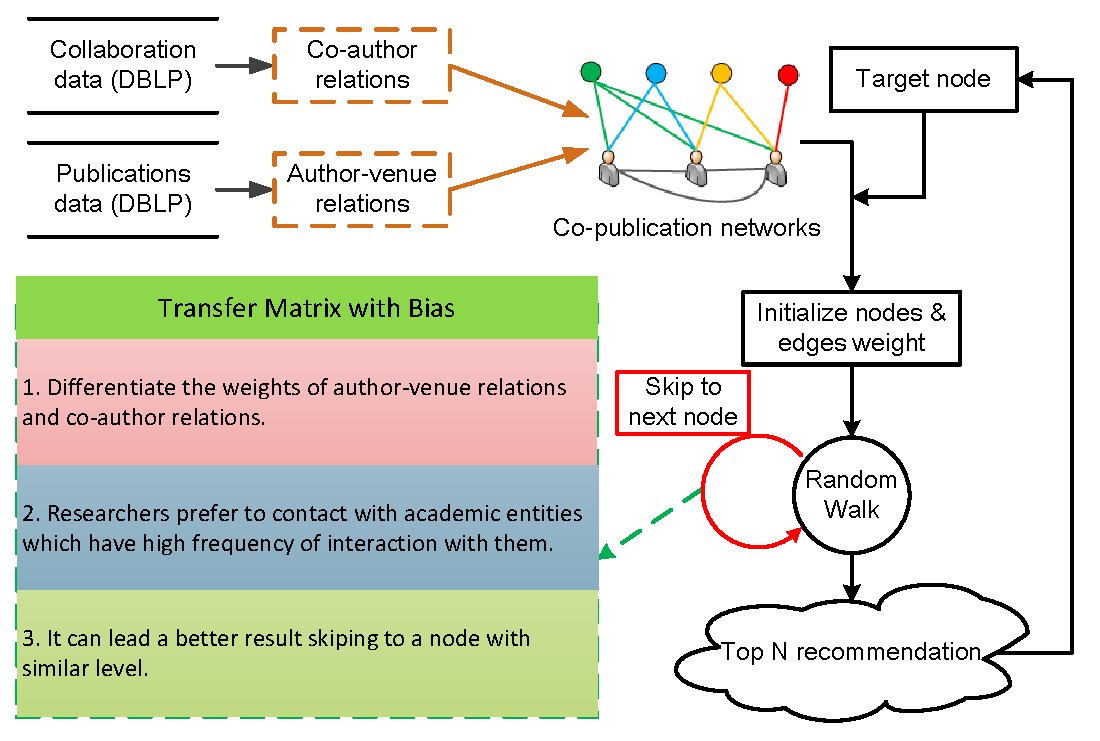
\includegraphics [width=3.2in]{Fig1.pdf}
\caption{The structure of AVER.}
\label{Fig1}
\end{figure}
\subsection{Overview of AVER}
In this work, we model a kind of co-publication networks which are characterized by researchers and academic venues. Figure~\ref{Fig2} shows an example of the network. The colorized nodes represent venues A, B, C and D. The three researchers Bob, David and Alice collaborate to write five papers which are published in the four venues respectively (note that Bob publishes two papers in venue A). The nodes (venues and researchers) along with links (co-author relations and author-venue relations) form the co-publication networks. We define two kinds of node sets, $Venues$ and $Authors$.
\begin{figure}[t]
\centering
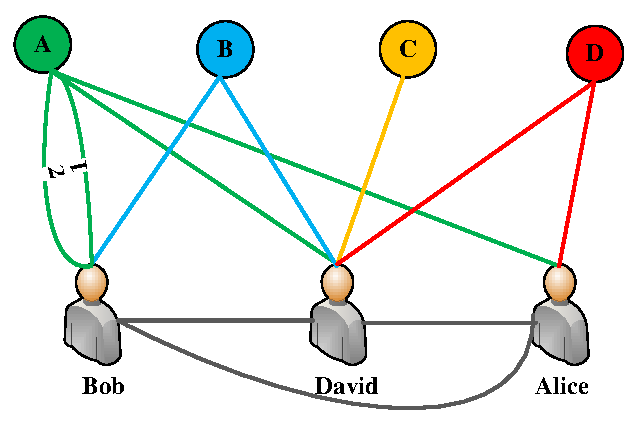
\includegraphics [width=2.5in]{Fig2.pdf}
\caption{An example of co-publication network}
\label{Fig2}
\end{figure}

In AVER, whether a venue should be recommended depends on its importance to the target researcher. The importance is defined by the rank score of the venue, which is determined by two factors, i.e. the number of neighbor nodes and the rank score of incident nodes. Equation~\ref{equ1} describes this theory.
\begin{equation}
\label{equ1}
AR(p_{i})=\frac{1-\alpha}{N}+\alpha \sum_{p_{j}\in A(p_{i})}AR(p_{j})P(p_{j},p_{i})
\end{equation}
$AR$ represents the rank score vector. $AR(p_{i})$ is the rank score of node $p_{i}$. $A(p_{i})$ is the set of nodes incident to node $p_{i}$. $P(p_{j},p_{i})$ is the transition probability from node $p_{j}$ to node $p_{i}$. $\alpha$ is the damping factor. When the AVER is running on the network to compute node ranking, starting from source node $p_{0}$, imaginary walker randomly walk in the network. The walker has two choice, i.e. with probability $\alpha$, walking to next node $p_{x}$, which is one of $p_{0}$'s direct neighbors ($p_{x}\in A(p_{0})$), or with probability $1-\alpha$, returning to source vertex $p_{0}$. Equation~\ref{equ1} represents one step to get rank score for node $p_{i}$. With respect to all nodes in the whole network, the approach is defined by equation~\ref{equ2}, which is an iterative process.
\begin{equation}
\label{equ2}
AR^{(t+1)}=\alpha \mathbf{S}AR^{(t)}+(1-\alpha)q
\end{equation}
$AR^{t}$ is the rank score vector at step $t$. $q$ is a row vector $(0,...,1,...,0)$. It should be noticed that, $AR_{0}=q$. The rank score of target node is $1$, while others' are $0$. $\mathbf{S}$ is the transfer matrix, representing the probability for each node to skip to next node. For basic RWR model, the cell of matrix $\mathbf{S}$ (i.e. $P(p_{j},p_{i})$ in Equation~\ref{equ1}) is defined as $\frac{1}{L(p_{i})}$. ($L(p_{i})$ is the number of node $p_{i}$'s neighbors). It means that, the walker has the same probability to skip to next node. In AVER, we do some guidance work by introducing three academic factors. The change of $P(p_{j},p_{i})$ can lead the walker skips with preference, which will be proved to be better in section~\ref{section:evaluation} for academic venue recommendation.

The detailed process of AVER is described below corresponding with the structure in Figure~\ref{Fig1}.

\begin{itemize}
  \item \emph{Step1}. The initial input data is a set of publications with authors' information and venues' information. AVER firstly extracts the co-author relations and author-venue relations, and then, generates the co-publication networks. There is a link between two authors if they coauthored at least one paper, as well as a link between researcher and venue if the researcher published a paper in the venue.
  \item \emph{Step2}. After initializing the rank score of nodes and weight of edges, AVER runs on the network. During the random walk process, the walker skips to next node with a modified probability by considering the three academic factors. The walk will stop until the rank score is approximately convergent or the iterations come to the upper limit.
  \item \emph{Step3}. After getting the convergent rank score of each node, AVER sorts the venue in accordance to their corresponding rank scores. Finally, removing the venues with which the target author has contacted, the Top-N venues are recommended to the target author.
\end{itemize}

We present the details below of how the transfer matrix with bias is computed by considering the three academic factors.

\subsection{Transfer Matrix with Bias}
As the example shown in Figure~\ref{Fig2}, there are seven academic entities. With respect to recommending venues to Bob, he has never contacted with venue C and D. According to the characteristics of the random walk with restart model, the walker can walk from Bob to C and D via David and Alice respectively. After several times iterative walking, venues C and D are recommended to Bob based on the sorted rank score. However, there are several academic factors that can be introduced to meet the real scene. We exploit three of them to redefine the transfer matrix in random walk with restart model.

Generally, researchers prefer contacting the academic entities (researchers and venues) which have high frequency of interaction with them, i.e. high publishing frequency in the venue or high collaborating frequency with the researchers. As shown in Figure~\ref{Fig2}, we think Bob prefers contacting David rather than Alice because Bob collaborated with David twice while Alice once. David seems to be more important than Alice for Bob. As well as Bob prefers contacting venue A rather than B, since Bob published two papers in venue A. Based on this assumption, We define co-publication frequency as Equation~\ref{equ3} which is a part of the links' weight.
\begin{equation}
\label{equ3}
F_{i,j}=\left\{\begin{array}{ll}
cp_{i,j} & i\in Author,\quad j\in Venues\\
ct_{i,j} & i,j\in Authors\\
\end{array}\right.
\end{equation}
Where $cp_{i,j}$ is the count of author $i$'s publications in venue $j$. $ct_{i,j}$ is author $i$'s collaborating times with author $j$.

In addition, there are two kinds of associations in co-publication networks, i.e. co-author relations and author-venue relations. In case of basic random walk model, the difference between these two relations is ignored. Author-venue relations seems to be more important than co-author relations, because the event of publishing a paper in the venue is more ponderable when profiling the researchers' interest. This proposition has been proved in subsequent experiments which can lead to better performance when making academic recommendation. We measure the weight of relations by Equation~\ref{equ4} based on a ratio $\beta$.
\begin{equation}
\label{equ4}
W_{i,j}=\beta F_{i,j}
\end{equation}
The ratio $\beta$ is a variable empirical value. In our experiments, $\beta$ is set as 20 for author-venue relations and 1 for co-author relations.

Finally, we proposed an assumption: the interest features of academic entities can be more accurately reflected by similar level neighbors. In case of researchers, they prefer contacting other researchers at similar academic levels and publishing papers in the venue which are more likely to accept the papers. In other words, the relations between similar-level academic entities are more weighty. The walker should walk along these nodes with more probability in AVER. In order to measure the similarity of academic entities, we define a simple metric as shown in equation~\ref{equ5}.
\begin{equation}
\label{equ5}
LevSim_{i,j}=1-\frac{\Vert AR_{i}-AR_{j}\Vert}{\max_{x\in L(i)}(\Vert AR_{i}-AR_{x}\Vert)}
\end{equation}
This equation~\ref{equ5} aims at discovering the neighbor with smallest rank score disparities based on a normalization method. When computing the transfer probability $S_{i,j}$ from node $i$ to node $j$, our AVER model adopts equation~\ref{equ6}. With equation~\ref{equ6}, the walker can run on the network with modified bias.
\begin{equation}
\label{equ6}
\mathbf{S}_{i,j}=\frac{W_{i,j}}{\sum_{x\in L(i)}W_{i,x}}LevSim_{i,j}
\end{equation}

\section{Evaluation and analysis}
\label{section:evaluation}
We conducted extensive experiments using data from DBLP~\cite{Ley:DBLP}, a computer science bibliography website hosted at University of Trier. In this section, we describe three academic venue recommendation approaches for comparison, the statistics of data set, the evaluation metrics and our experimental procedure for evaluating the performance of AVER, as well as detailed analysis of the results.

\subsection{Three Comparison Approaches}
To measure the performance of AVER, we conducted three comparison approaches, i.e. the basic random walk with restart model (RWR), a topic-based model and a friends-based model.

Similar to popular random walk models, the details and verification method of RWR is just like AVER, except for the definition of transfer matrix with bias. The topic-based method is a content-based recommendation approach in the strict sense. The core of the approach is to compute the similarity between researchers and venues. In this implementation, we regard the topic distribution of researchers' publications content and venues's publications content as feature vector respectively, which are calculated by LDA(Latent Dirichlet Allocation) model~\cite{blei2003latent}. The similarity of researchers and venues is defined by the Cosine Similarity based on these feature vectors. The friends-based model is a kind of collaborative filtering recommendation approach. Its basis of recommending venues is the number of neighbors who have relations with the venues. In this implementation, we treat researcher's collaborators and "collaborators of collaborator" as neighbors. If there are many neighbors contact a venue, the venue should be recommended to the researcher.

\subsection{Data Set and Metrics}
DBLP indexes more than 2.3 million articles on computer science. In our experiments, we use a subset of DBLP. The subset data are all in the field of data mining involving 34 journals and 38 conferences altogether. The statistics about the data sets are shown in Table~\ref{table1}. The data set contains 74 venues and 70326 researches. 163446 articles connected researchers and venues, as well as came into being the co-publication networks. We divided the data set into two parts: the data before year 2011 as a training set, and others as a testing set.
\begin{table}
\renewcommand{\arraystretch}{1.2}
\centering
\caption{Statistics of Data Set from DBLP}
\label{table1}
\begin{tabular}{|c|c|c|c|} \hline
Statistics &venues&researchers&articles\\ \hline
Number & 74 & 70326 &163446 \\
\hline\end{tabular}
\end{table}

\begin{figure}[t]
\centering
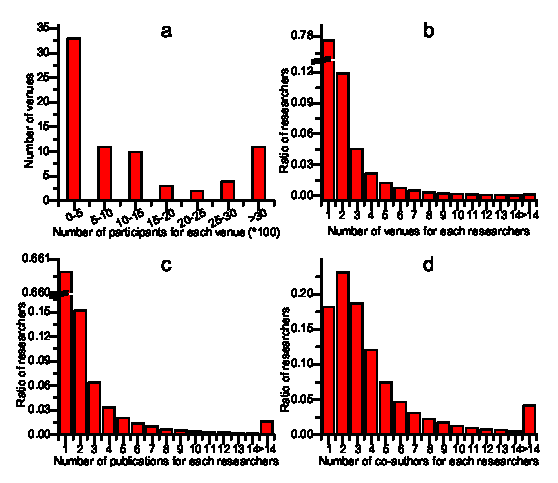
\includegraphics [width=3.5in]{Fig3.eps}
\caption{Detailed statistics of the data set from DBLP}
\label{fig3}
\end{figure}
\begin{figure*}[hbt]
\centering
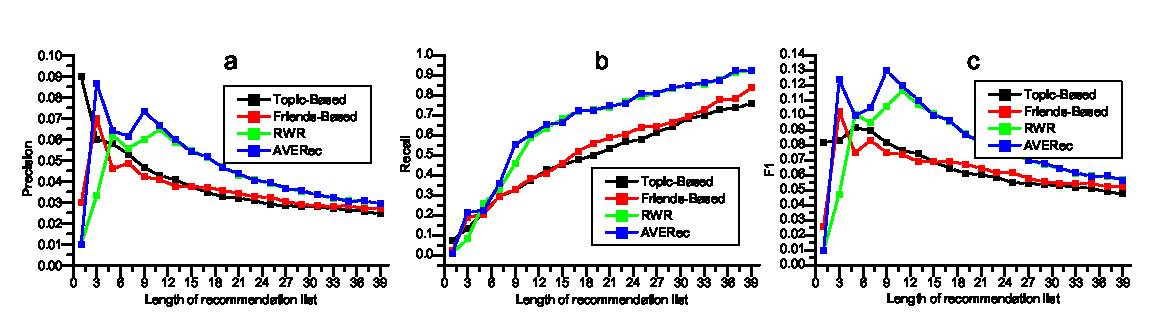
\includegraphics [width=\textwidth]{Fig4.eps}
\caption{Performance of AVER, basic RWR, topic-based and friends-based recommendation model}
\label{fig4}
\end{figure*}
\begin{figure*}[hbt]
\centering
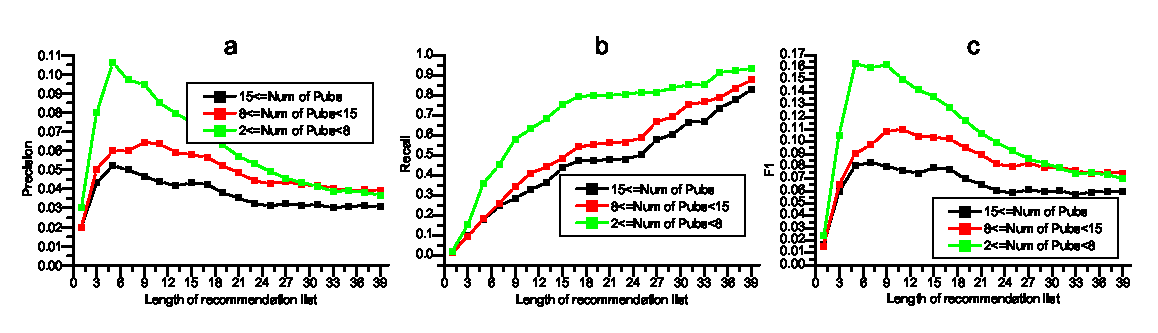
\includegraphics [width=\textwidth]{Fig5.eps}
\caption{The impact of researchers' publications number on AVER}
\label{fig5}
\end{figure*}

The detailed statistical characteristic of this co-publication network is shown in Figure~\ref{fig3}. Figure~\ref{fig3}(a) describes the scale of participants or contributors for each venue. Almost half of the venues keep not more than 500 researchers. The scale of 11 venues is so large that up to 3000 researchers publish papers on them. We can also get that from Figure~\ref{fig3}(b), almost $94$ percentage of these 70326 researchers contact not more than 3 venues. However, there are also some "academic stars" (account for $0.13\%$) contributing more than 14 venues. Similarly, Figure~\ref{fig3}(c) shows the same trend for the number of researchers' publications. Most of them published not more than five papers, but there were also many researchers publishing more than 14 papers. Figure~\ref{fig3}(d) shows the number of co-authors for each researchers. We can conclude that, the degrees of most researchers are under 14, which indicates that this data set is very sparse.

We use three popular metrics, precision, recall and F1 score, to evaluate the performance of AVER. Detailed information about these metrics has been discussed in~\cite{xia2014mvcwalker}. All experiments were performed on a 64-bit Linux-based operation system, Ubuntu 12.04 with a 4-duo and 3.2-Ghz Intel CPU, 8-G Bytes memory, and implemented with Python.

\subsection{Results and Analysis}
In this section, we firstly conducted several experiments for AVER, basic RWR, topic-based and friends-based recommendation model on aforesaid data set. Secondly, we measured the performance of AVER when recommending academic venues for researchers at different levels. We randomly chose 100 researchers as target nodes. Additionally, AVER and RWR were run with the damping factor 0.8.

Figure~\ref{fig4} shows the performance of AVER, basic RWR, topic-based and friends-based recommendation model. The $x$ axis represents the length of recommendation list, which were range in 1 to 39. The $y$ axis represents precision, recall and F1 score respectively. In case of Figure~\ref{fig4}(a), all lines roughly show coincident downtrend. However, AVER and basic RWR performed better in precision as a whole. On the view of range 1 to 11 on $x$ axis, AVER gets higher precision, as well as that it comes to a peak value $8.7\%$ at point 3. With the growth of recommendation list, the performance of the four recommendation approach tends to be similar. In case of Figure~\ref{fig4}(b), the lines rise obviously. AVER and basic RWR have no significant difference, but their recall performed better than that of topic-based and friends-based approach. With the number of recommended venues reaching to the sum of venues, the recall approximates to 1. According to Figure~\ref{fig4}(c), the F1 score shows similar trend with precision. The F1 score of AVER reaches the highest value of $12.95\%$ when recommending 9 venues for each researchers. The upgrade rate ($\frac{F1(AVER)-F1(RWR)}{F1(RWR)}$) is $11.3\%$ comparing to basic RWR. It is worth mentioning that, AVER reaches its peak at point 9, while basic RWR gets highest F1 score at point 11. That means the recommendation efficiency of AVER is higher.

These experiments demonstrated that, the random walk with restart based model can get more accurate academic venue recommendation than topic-based and friends-based approaches. What's more, our work on transfer matrix with bias does improve the performance of AVER, and makes the recommendation more efficient.

We also made several extensive experiments to measure the performance of AVER on different researchers. We mainly focused on the difference of researchers academic level, which is reflected by the number of publications. Generally, the newcomer shows lower academic level with few publications, while a fruitful professor shows high academic level with a plenty of high-quality publications. We divided the researchers into three sets, i.e. $C1$ contains researchers whose publications number range from 2 to 8, $C2$ contains researchers with 8 to 15 publications and $C3$ contains researchers with more than 15 publications. The experimental results are show in Figure~\ref{fig5}.

From Figure~\ref{fig5}, we can see significant difference of the effect on different sets of researchers even though they show a similar trend in precision, recall and F1 score respectively. In Figure~\ref{fig5}(c), the AVER can get highest value $16.24\%$ for F1 score at point 9 when making academic venue recommendation for the researchers with 2 to 8 publications. The results mean that, AVER can do better at recommending academic venues for researchers with fewer publications, i.e. the relatively newcomer, which meets our original intention of recommending academic venues well for the newcomer.

\section{Conclusions}
In this paper, we focused on academic venue recommendation for researchers based on the big scholarly data which is necessary in current academia. To this end, we proposed a novel academic venue recommendation model called AVER, which exploits three academic factors (i.e. co-publication frequency, weight of relations and researchers' academic level) to define transfer matrix with bias which drives a random walk with restart model running on the co-publication network. We conducted extensive experiments on a subset of DBLP data set to evaluate the performance of AVER in comparison to other state-of-the-art approaches: basic RWR, topic-based approaches and friends-based approaches. The experimental results show that, AVER outperforms other approaches in terms of precision, recall and F1 score. According to the extended experiment, AVER performs better at recommending academic venues for researchers with fewer publications, i.e. the relatively newcomer.

Nonetheless, there is still room for future study in this direction. We only exploited three academic factors in co-publication network. There are also many other features. For instance, citation relations should be explored which has been incorporated in venue recommendation by Onur~\cite{kuccuktuncc2012recommendation}. As a future work, more experiments should be conducted on other academic data sets.
%\end{document}  % This is where a 'short' article might terminate

%ACKNOWLEDGMENTS are optional
%\section{Acknowledgments}

\bibliographystyle{unsrt}
\bibliographystyle{abbrv}
\bibliography{AVER}
%\appendix
%Appendix A
\balancecolumns
\end{document}
